\chapter{Implementation and Technical Realization}
\minitoc
\newpage

\setcounter{secnumdepth}{0} % Set the section counter to 0 so next section is not counted in toc
% ----------------------- Introduction ----------------------- %
\section{Introduction}
This chapter covers the practical implementation of the architecture 
designed in the previous chapter. The work follows a bottom-up approach, 
starting from containerizing the applications, configuring the Kubernetes 
cluster, provisioning the cloud infrastructure with Terraform, and finally 
setting up the CI/CD pipelines that automate the entire delivery process.

\setcounter{secnumdepth}{3}

% ----------------------- Kubernetes Configuration ----------------------- %
\section{Container Orchestration and Kubernetes Deployment}
As mentioned previously, The Mashroom platform is implemented by containerizing each application 
into a Docker image and orchestrating them using Kubernetes. All cluster 
configuration is stored in a dedicated GitOps repository and validated 
locally using Minikube before targeting the cloud environment.

% ----------------------- Containerization ----------------------- %
\subsection{Application Containerization}
The Mashroom platform is composed of three applications: the 
backend API, the Studio interface, and the Landing Page. Each 
one is packaged into a Docker container image so it runs the 
same way locally and in the cloud.

For this reason, we create three dockefiles that follow a multi-stage build pattern to keep the 
final images as small as possible.

Figure \ref{fig:studio-df} illustrates the Studio Dockerfile, the most 
complex of the three. It adds extra build tools to compile native C++ 
modules and accepts build arguments for the API URL and key, which are 
injected before the app is served through Nginx.

\begin{figure}[H]
    \centering
    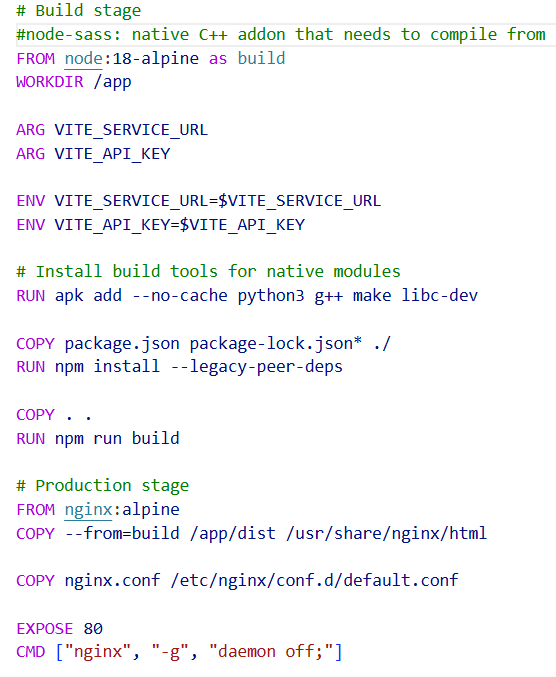
\includegraphics[width=0.6\linewidth]{src/assets/screenshots/studio-df.png}
    \caption{Multi-stage Dockerfile for Studio}
    \label{fig:studio-df}
\end{figure}

\subsection{GitOps Repository Structure} 
The GitOps repository is organized into three main directories, 
as illustrated in figure \ref{fig:gitops-structure}. The \texttt{apps} 
directory contains the base Kubernetes manifests as well as the Kustomize 
overlays used for each environment. The \texttt{secrets} directory stores 
the External Secrets Operator resources responsible for retrieving 
credentials from AWS Secrets Manager and injecting them into the cluster. 
Finally, the \texttt{argocd} directory contains the ArgoCD application 
definitions, which specify what ArgoCD should deploy and in which target 
environment.

\begin{figure}[H]
    \centering
    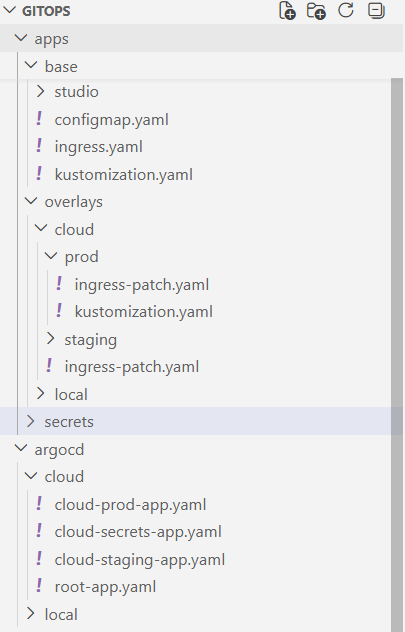
\includegraphics[width=0.5\linewidth]{src/assets/screenshots/gitops-structure.png}
    \caption{GitOps repository structure}
    \label{fig:gitops-structure}
\end{figure}

\subsubsection*{\underline{Application Manifests and Environment Separation}}
Inside the \texttt{apps} directory, the \texttt{base} folder contains 
the Kubernetes manifests shared across all environments. These manifests 
include a Deployment, an Ingress, and a ConfigMap for each application. 
The Deployment manifest, shown in figure \ref{fig:deployment-manifest}, 
defines the API pod configuration, including the container image pulled 
from GitHub Container Registry (GHCR), the exposed port, and the references to configuration values 
and secrets injected into the container at runtime.

\begin{figure}[H]
    \centering
    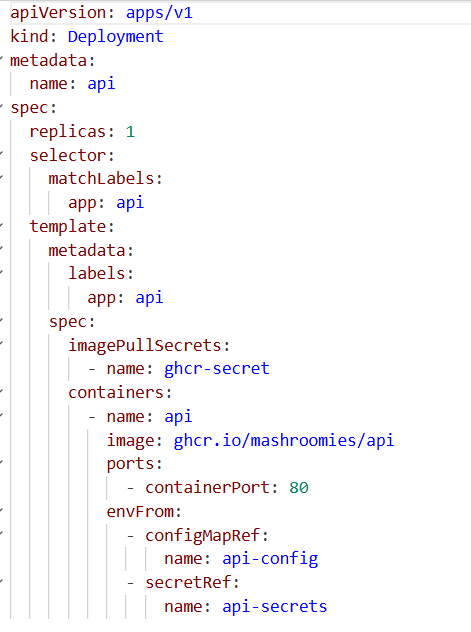
\includegraphics[width=0.65\linewidth]{src/assets/screenshots/deployment-manifest.png}
    \caption{Base Deployment manifest for the backend API}
    \label{fig:deployment-manifest}
\end{figure}

The ConfigMap, presented in figure \ref{fig:configmap-manifest}, stores 
the non-sensitive configuration parameters of the API, such as database 
connection information, JWT expiration settings, and the AWS region.

\begin{figure}[H]
    \centering
    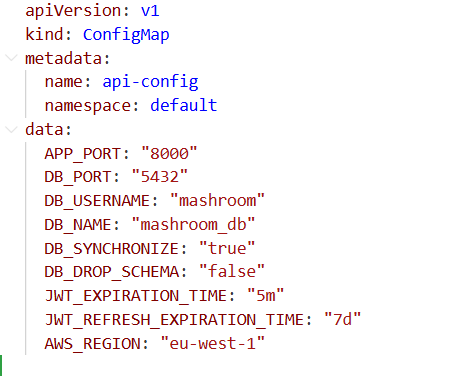
\includegraphics[width=0.75\linewidth]{src/assets/screenshots/configmap-manifest.png}
    \caption{ConfigMap holding the API configuration values}
    \label{fig:configmap-manifest}
\end{figure}
To support multiple environments without duplicating manifests, the 
project relies on Kustomize overlays. These overlays extend the base 
manifests while keeping the original files unchanged. The repository 
is divided into two overlay groups: \texttt{local}, dedicated to local 
development using Minikube, and \texttt{cloud}, used for the environments 
deployed on EKS. Each group contains two environments: \texttt{prod} 
and \texttt{staging}.

Each Kustomize overlay has three main responsibilities. First, it defines 
the target namespace in order to isolate each environment inside the 
cluster. Second, it patches the Ingress resource so that each environment 
uses the appropriate hostname. Third, it overrides the image tags to 
deploy a specific version of the application in each environment.

In addition, the staging overlay sets the replicas of the Studio and 
Landing Page to zero, since only the API is required in this environment. 
This reduces resource consumption while still allowing the environment 
to be activated easily by increasing the replica count when needed.

\subsubsection*{\underline{Secrets Injection with External Secrets Operator}}
Sensitive credentials are never stored directly in the GitOps repository. 
Instead, the External Secrets Operator retrieves them securely from AWS 
Secrets Manager and injects them into the cluster as native Kubernetes secrets.

To achieve this, a \texttt{ClusterSecretStore} resource is first configured 
to establish the connection with AWS Secrets Manager through the External 
Secrets Operator service account. Then, two \texttt{ExternalSecret} resources 
are defined. The first creates the \texttt{api-secrets} Kubernetes secret, 
which contains the database password, JWT secret, and S3 access keys. The 
second creates the \texttt{ghcr-secret}, used by the cluster to authenticate 
and pull container images from GHCR. As illustrated in figure 
\ref{fig:external-secrets}, both secrets are automatically refreshed every 
hour to ensure synchronization with AWS Secrets Manager.

\begin{figure}[H]
    \centering
    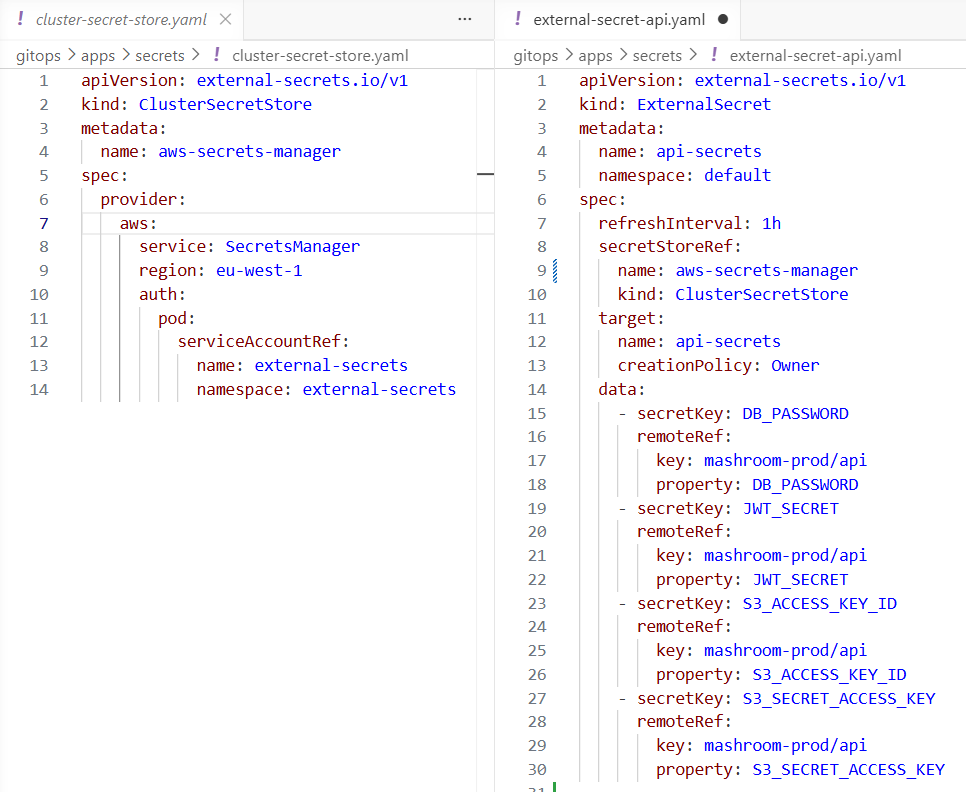
\includegraphics[width=0.9\linewidth]{src/assets/screenshots/cluster-secret-store.png}
    \caption{ExternalSecret resources pulling credentials from AWS Secrets Manager}
    \label{fig:external-secrets}
\end{figure}


% ----------------------- Infrastructure Provisioning ----------------------- %
\section{Infrastructure Provisioning with Terraform}
The AWS cloud infrastructure hosting the Mashroom applications is 
provisioned using Terraform, with all resources defined as code and 
organized into modules, each responsible for a separate part of the 
infrastructure. Each module is detailed below, followed by a validation 
of the provisioned resources.

\subsection{Project Structure and Module Organization}
The Terraform codebase is structured around a root environment 
directory and a set of child modules as shown in figure 
\ref{fig:terraform-modules-struture}. The root directory contains the 
entry point files such as \texttt{main.tf}, \texttt{variables.tf}, 
and \texttt{providers.tf}. Each module under the \texttt{modules/} 
directory is responsible for a distinct AWS component: \texttt{network} 
for the VPC, \texttt{eks} for the cluster, \texttt{rds} for the 
database, \texttt{s3} for file storage, \texttt{secrets} for 
credentials management, and \texttt{k8s-workloads} for cluster-level resources.

\begin{figure}[H]
    \centering
    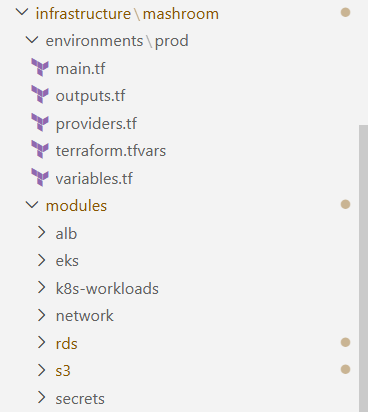
\includegraphics[width=0.7\linewidth]{src/assets/images/terraform-modules.png}
    \caption{Terraform project structure with modular organization}
    \label{fig:terraform-modules-struture}
\end{figure}

\subsection{Network Configuration}
The network module provisions a Virtual Private Cloud (VPC) that 
acts as the boundary for the entire infrastructure. Two types of 
subnets are created inside it: public subnets that host the 
Internet Gateway, which enables inbound traffic from the internet, 
and the Application Load Balancer, which routes external requests 
to the cluster. Private subnets host the EKS cluster nodes and 
the RDS database instance, keeping them inaccessible from the public internet.

\begin{figure}[H]
    \centering
    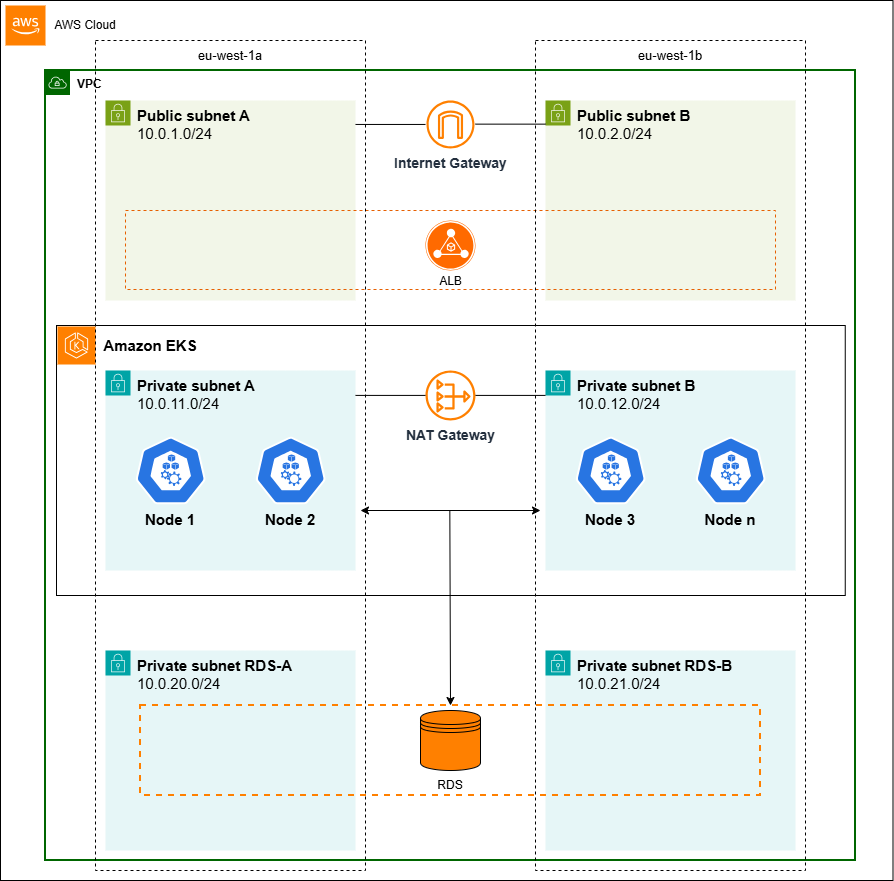
\includegraphics[width=0.7\linewidth]{src/assets/diagrams/network.png}
    \caption{Network architecture showing VPC, subnets, and AWS components}
    \label{fig:network-arch}
\end{figure} 

Outbound traffic from the private subnets reaches the internet 
through the NAT Gateway, which is necessary for the cluster nodes 
to pull application images from the GitHub Container Registry.

\subsection{EKS Cluster Provisioning}
The \texttt{eks} module provisions the Kubernetes cluster and its worker 
nodes inside the private subnets of the VPC.

\begin{figure}[H]
    \centering
    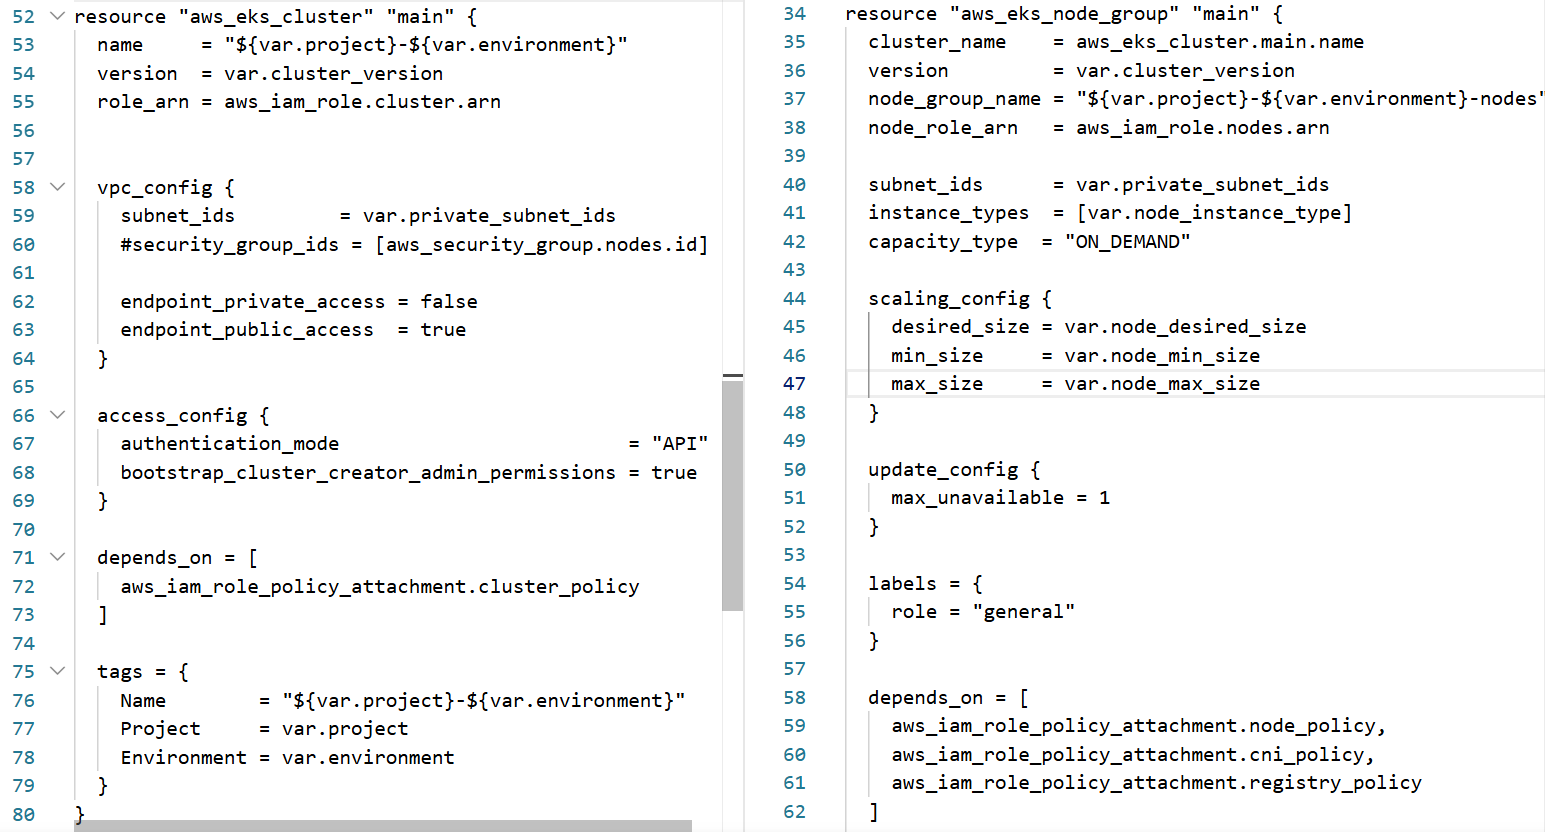
\includegraphics[width=1\linewidth]{src/assets/screenshots/eks-cluster-node-tf.png}
    \caption{Terraform resource definitions for the EKS cluster and node group}
    \label{fig:eks-cluster-tf}
\end{figure}

As shown in Figure \ref{fig:eks-cluster-tf}, the cluster is configured with 
a specific Kubernetes version, placed inside the private subnets, and kept 
private from the public internet.

The node group specifies the instance type, capacity type, and a scaling 
configuration that allows the cluster to automatically adjust the number 
of running nodes based on demand.


\subsection{RDS, S3, and Secrets Manager}
Beyond the cluster itself, three additional AWS services are 
provisioned to handle data persistence, file storage, and 
credential management.

The \texttt{rds} module provisions a managed PostgreSQL database 
instance placed inside the dedicated private subnets, configured 
with allocated storage limits, backup retention, and deletion 
protection. The \texttt{s3} module provisions a dedicated assets 
bucket for storing media and 3D files, allowing clients to upload 
and fetch content directly without routing through the cluster. 
The \texttt{secrets} module creates two secret entries in AWS 
Secrets Manager: one for the backend API credentials and one 
for the GHCR authentication token used by the cluster to pull 
application images. The Terraform resource definitions for all 
three modules are shown in figure \ref{fig:aws-services-tf}.

\begin{figure}[H]
    \centering
    \begin{subfigure}[t]{0.32\linewidth}
        \centering
        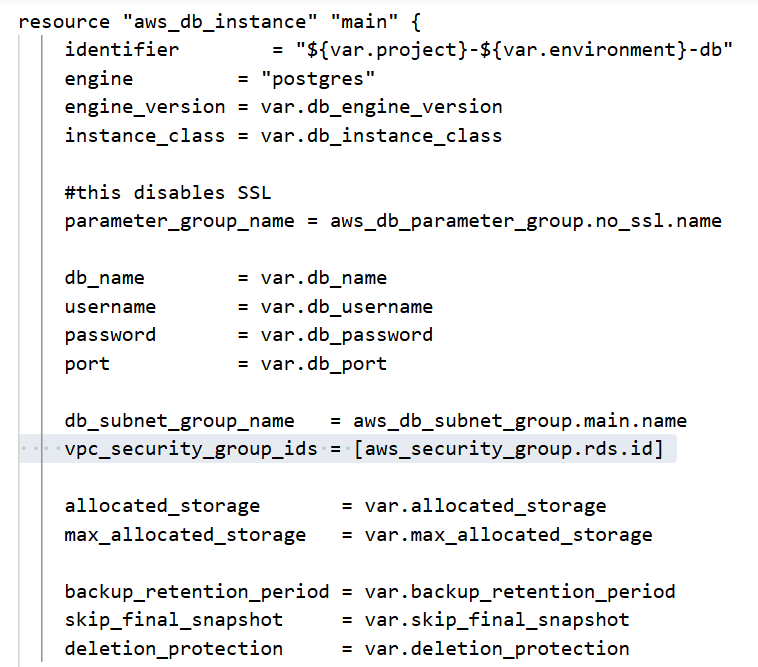
\includegraphics[width=\linewidth]{src/assets/screenshots/rds.png}
        \caption{RDS instance}
        \label{fig:rds-tf}
    \end{subfigure}
    \hfill
    \begin{subfigure}[t]{0.32\linewidth}
        \centering
        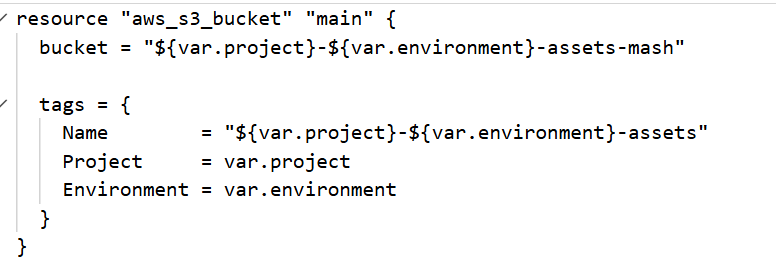
\includegraphics[width=\linewidth]{src/assets/screenshots/s3.png}
        \caption{S3 bucket}
        \label{fig:s3-tf}
    \end{subfigure}
    \hfill
    \begin{subfigure}[t]{0.32\linewidth}
        \centering
        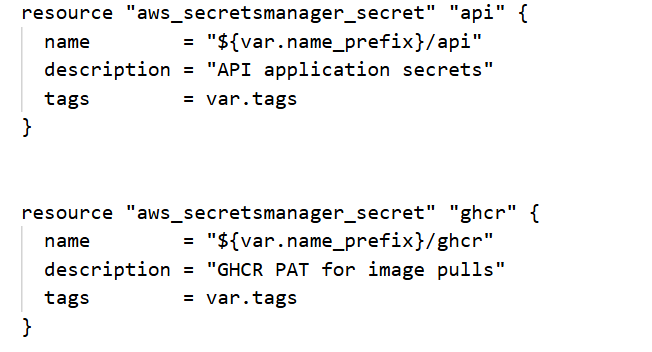
\includegraphics[width=\linewidth]{src/assets/screenshots/secrets.png}
        \caption{Secrets Manager}
        \label{fig:secrets-tf}
    \end{subfigure}
    \caption{Terraform resource definitions for RDS, S3, and Secrets Manager}
    \label{fig:aws-services-tf}
\end{figure}

\subsection{Terraform Plan Verification}
Before applying the infrastructure, the \texttt{terraform plan} 
command was run to preview all the resources that would be created. 
As shown in figure \ref{fig:terraform-plan}, the output confirms 
that all expected resources were planned with no errors.

\begin{figure}[H]
    \centering
    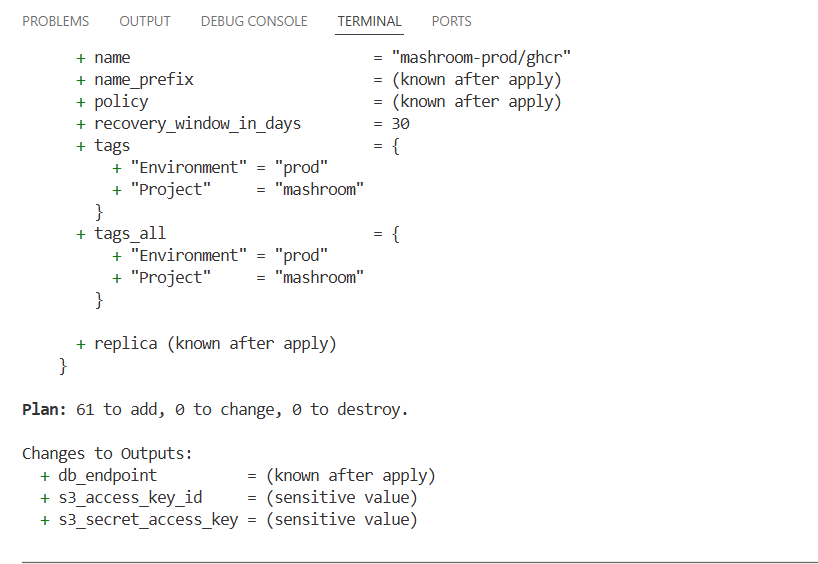
\includegraphics[width=0.85\linewidth]{src/assets/screenshots/tf-plan.png}
    \caption{Terraform plan output showing the planned resources}
    \label{fig:terraform-plan}
\end{figure}

\subsection{Cluster and Node Health}
Once the infrastructure was applied, the cluster and its nodes 
were verified to be in a healthy state. As shown in figures 
\ref{fig:cluster-health} and \ref{fig:node-health}, all nodes are in \texttt{Ready} status, 
confirming the cluster is operational and ready to receive workloads.

\begin{figure}[H]
    \centering
    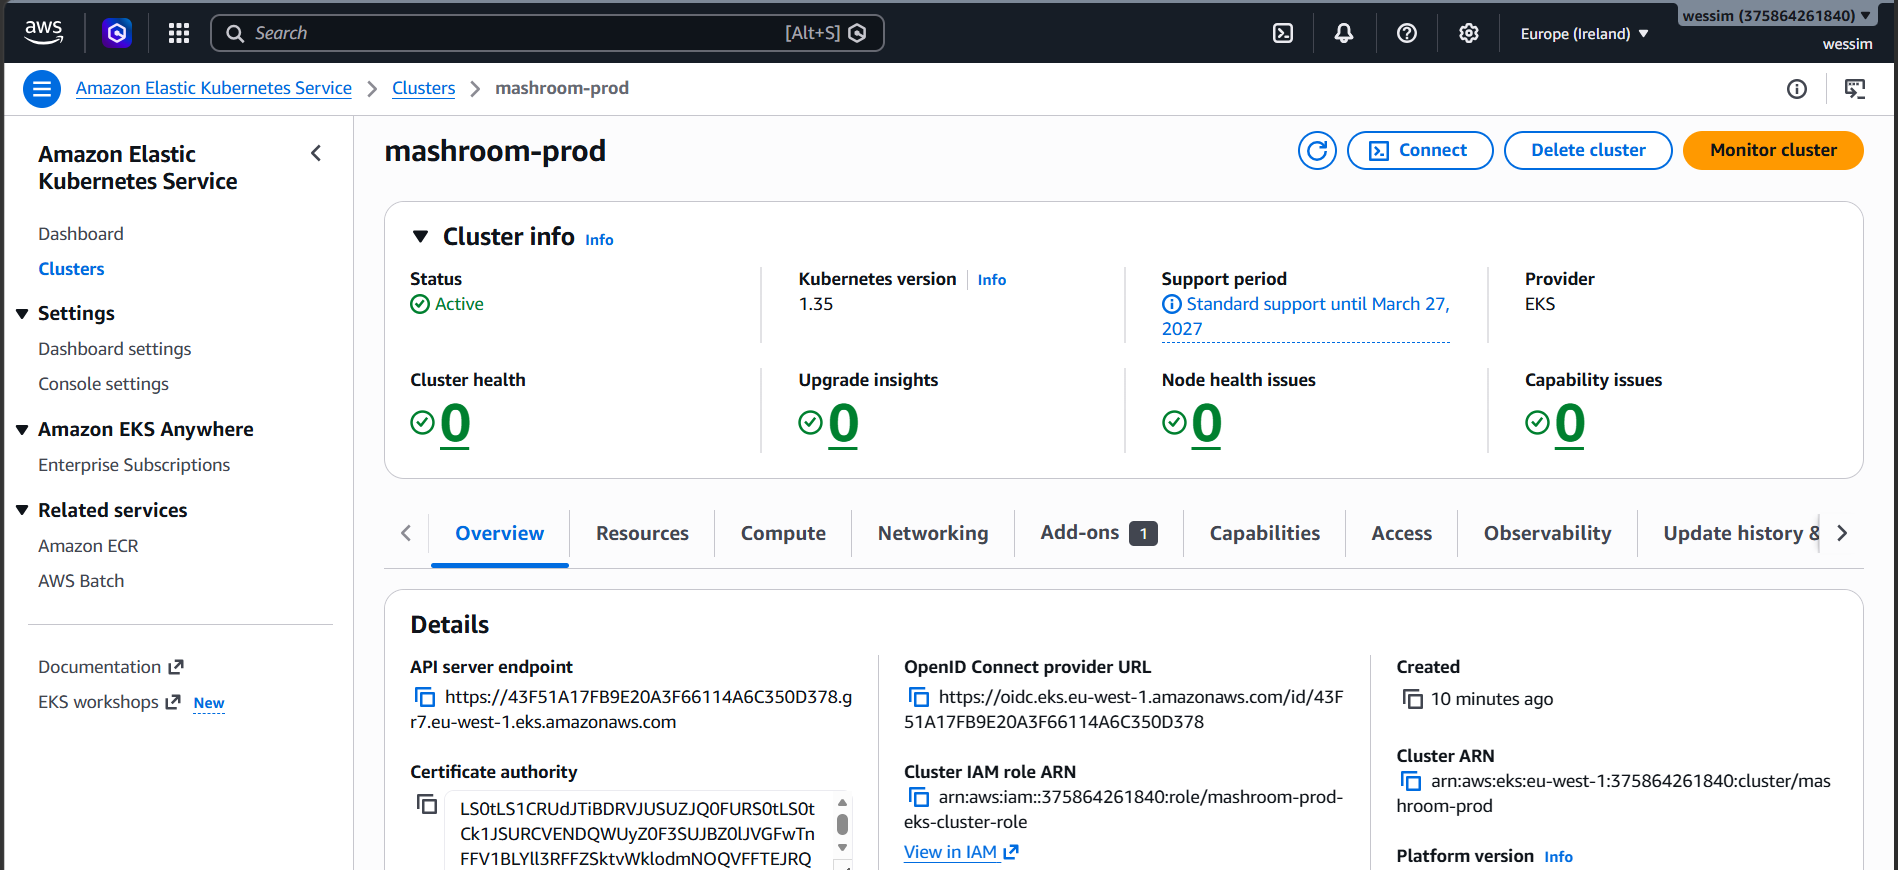
\includegraphics[width=1\linewidth]{src/assets/screenshots/eks-health.png}
    \caption{Cluster nodes in Ready state after provisioning}
    \label{fig:cluster-health}
\end{figure}

\begin{figure}[H]
    \centering
    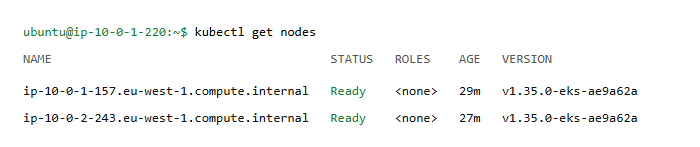
\includegraphics[width=1\linewidth]{src/assets/screenshots/node-health.png}
    \caption{Worker nodes in Ready state following EKS cluster provisioning}
    \label{fig:node-health}
\end{figure}

\section{CI/CD Pipeline Implementation}
This section covers the implementation of the full CI/CD pipeline 
that automates the delivery of The Mashroom's applications. It is 
divided into two parts: the Continuous Integration pipeline built 
with GitHub Actions, which handles code quality checks, image builds, 
and registry pushes, and the Continuous Deployment setup powered by 
ArgoCD, which ensures the cluster always reflects the latest state 
of the GitOps repository. The section concludes with a validation 
of the end-to-end pipeline behavior.

% ----------------------- CI ----------------------- %
\subsection{Continuous Integration with GitHub Actions}
As established in Section 2.3.3, GitHub Actions was selected to automate 
the build and delivery of The Mashroom's three applications.
This section covers the practical implementation of the CI pipelines, 
following the workflow illustrated in figure \ref{fig:ci-pipeline}.

\subsubsection*{\underline{Pipeline Structure and Triggers}}
The three applications share the same branching strategy but 
differ slightly in behavior:

\begin{itemize}
    \item \textbf{Pull request to \texttt{develop}:} the image 
    is built and saved locally on the runner tagged with the 
    commit SHA (a unique identifier generated for each commit), 
    without pushing to GHCR.
    
    \item \textbf{Merge into \texttt{develop}:} the API and 
    Studio images are built and pushed to GHCR tagged with 
    the commit SHA and \texttt{dev}. The Landing Page has no 
    develop branch and is only built on merge into \texttt{main}.
    
    \item \textbf{Merge into \texttt{main}:} all three images 
are pulled from GHCR, retagged as \texttt{main}, and pushed 
back. Each pipeline then updates the image tags in the GitOps 
repository for the production environment, while the develop 
branch targets the staging environment.
\end{itemize}

\subsubsection*{\underline{Code Quality and Tests}}
Each pipeline run starts with a linting step that checks the 
code for formatting and syntax errors before the image is built, 
ensuring that no malformed code reaches the registry. Unit and 
integration tests are to be added in a future iteration of the 
pipeline.

\subsubsection*{\underline{Image Build and Push to GHCR}}
Once the pipeline completes successfully, the built images are 
available in the GitHub Container Registry ready to be used as shown in figure 
\ref{fig:ghcr-images}.

\begin{figure}[H]
    \centering
    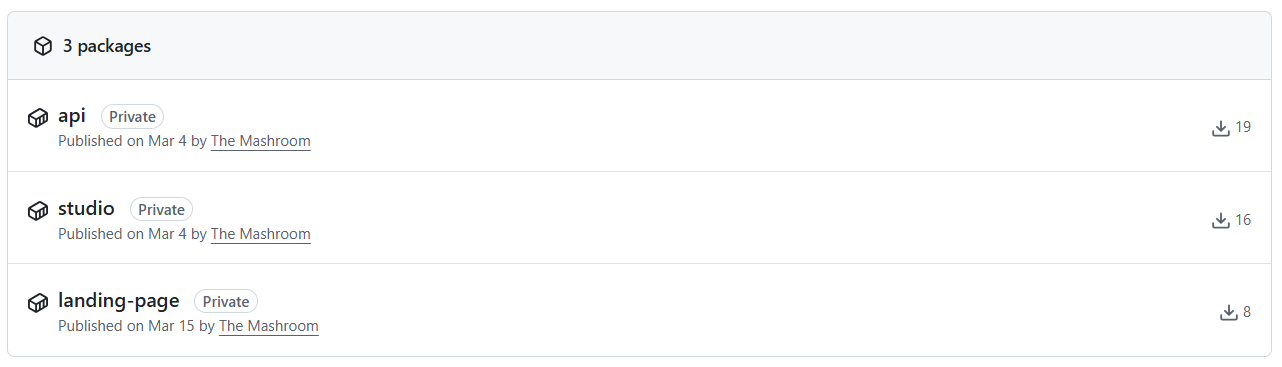
\includegraphics[width=1\linewidth]{src/assets/screenshots/ghcr-images.png}
    \caption{Application images stored in the GitHub Container Registry}
    \label{fig:ghcr-images}
\end{figure}

\subsubsection*{\underline{Automated Image Tag Update in the GitOps Repository}}
Once the image is pushed to GHCR, the pipeline automatically 
updates the GitOps repository to reflect the new version. As 
shown in figure \ref{fig:gitops-update}, the job checks out 
the GitOps repository, uses Kustomize to update the image tag 
in both the local and cloud overlays for the target environment, 
and commits the changes back to the repository. This commit is 
what triggers ArgoCD to detect a change and sync the cluster 
to the new version.

\begin{figure}[H]
    \centering
    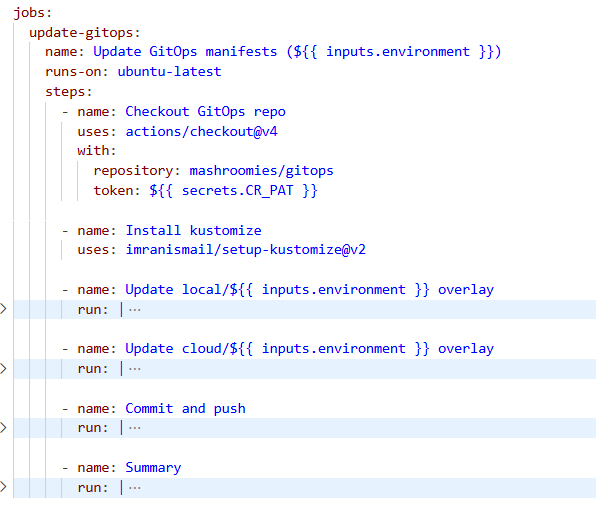
\includegraphics[width=0.9\linewidth]{src/assets/screenshots/gitops-update.png}
    \caption{GitOps update job in the GitHub Actions workflow}
    \label{fig:gitops-update}
\end{figure}

\subsubsection{GitHub Actions Workflow Results}
Figure \ref{fig:gh-actions-results} shows a successful pipeline
run triggered by a push to \texttt{main}. The build job
completed in 40 seconds and the GitOps update job ran
immediately after, confirming that the image tag was
automatically updated in the GitOps repository.
 
\begin{figure}[H]
    \centering
    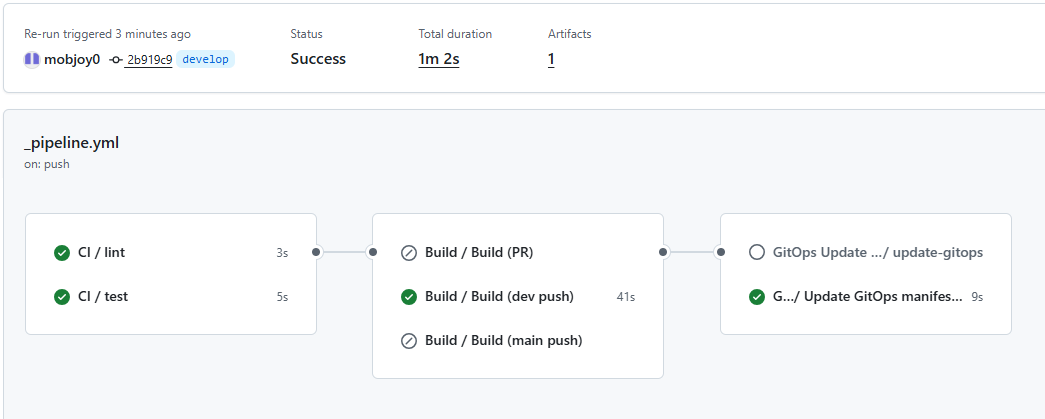
\includegraphics[width=0.9\linewidth]{src/assets/images/gh-actions-results.png}
    \caption{Successful GitHub Actions pipeline run}
    \label{fig:gh-actions-results}
\end{figure}

% ----------------------- CD ----------------------- %
\subsection{Continuous Deployment with ArgoCD}
With the CI pipelines in place, the final step is automating 
how changes reach the cluster. This section covers the setup 
of ArgoCD as the GitOps delivery tool responsible for keeping 
the cluster in sync with the GitOps repository.

\subsubsection*{\underline{ArgoCD Installation and Configuration}}
ArgoCD is installed into the cluster using Helm, a package 
manager for Kubernetes that simplifies the deployment of 
third-party applications by bundling all the necessary 
manifests into a single installable package. As shown in 
figure \ref{fig:argocd-helm}, the installation is managed 
through Terraform using the \texttt{helm\_release} resource, 
which pulls the official ArgoCD chart and installs it into 
a dedicated \texttt{argocd} namespace inside the cluster.

\begin{figure}[H]
    \centering
    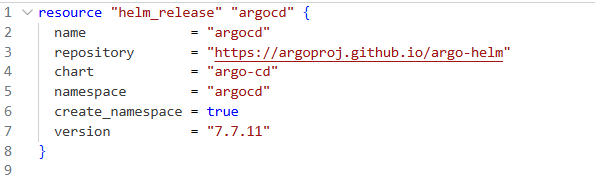
\includegraphics[width=1\linewidth]{src/assets/screenshots/argocd-helm.png}
    \caption{ArgoCD installation using Helm in Terraform}
    \label{fig:argocd-helm}
\end{figure}

\subsubsection*{\underline{Application Definitions and Synchronization Policies}}
ArgoCD is configured using the app of apps pattern. Instead of 
manually registering each application in ArgoCD, a single root 
application is defined that watches the \texttt{argocd/cloud} 
directory in the GitOps repository. When ArgoCD detects a change 
in that directory, it automatically creates or updates all the 
other applications defined inside it.

Figure \ref{fig:argocd-apps} shows both the root and the production 
application definitions. The root application is configured with two 
important Synchronization options:

\begin{itemize}
    \item \texttt{prune}: removes cluster resources when they are 
    deleted from the repository.
    \item \texttt{selfHeal}: reverts any manual changes made directly 
    in the cluster back to the repository state.
\end{itemize}

Each child application points to a specific Kustomize overlay and 
deploys into its own dedicated namespace, keeping environments fully 
isolated from each other.

\begin{figure}[H]
    \centering
    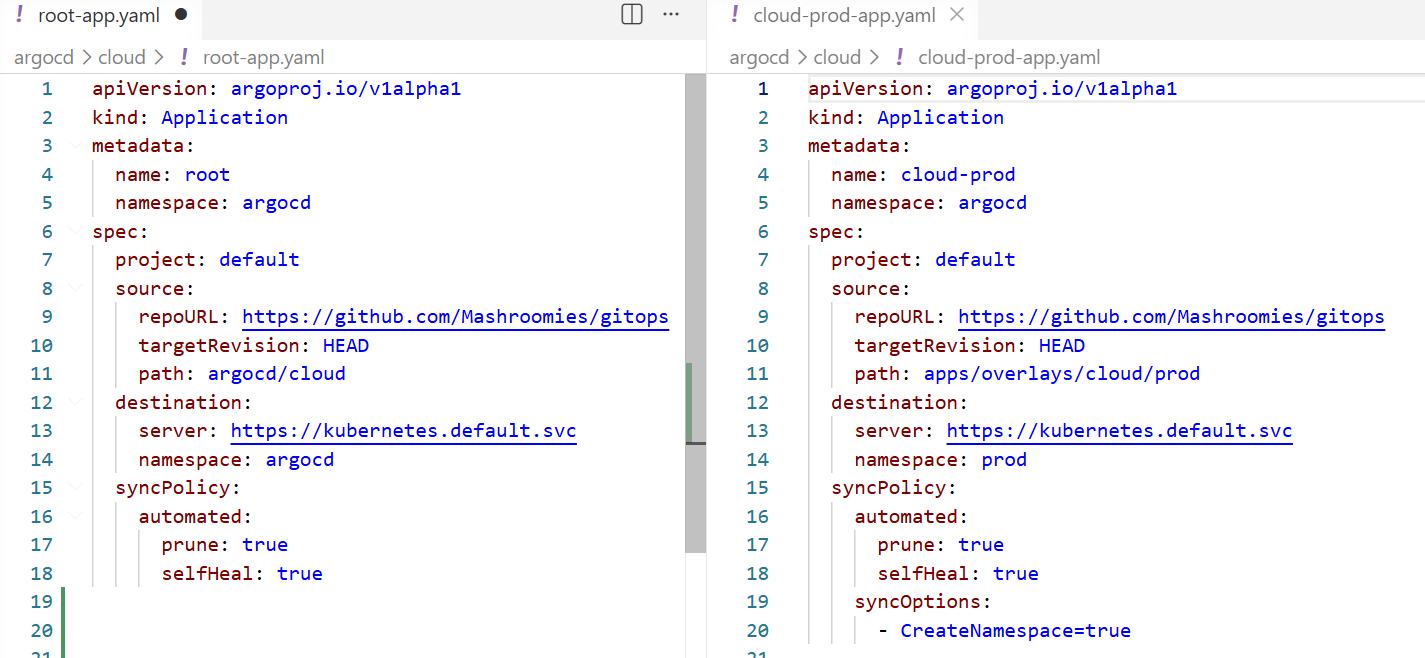
\includegraphics[width=1\linewidth]{src/assets/screenshots/argocd-apps.png}
    \caption{Root and production ArgoCD application definitions}
    \label{fig:argocd-apps}
\end{figure}

\subsubsection*{\underline{Automated Rollbacks}}
Because the cluster state is entirely driven by the GitOps repository, 
rolling back a bad release requires no manual intervention on the cluster. 
Reverting a commit in the repository is enough to restore the previous 
state. ArgoCD detects the change and automatically re-syncs the cluster 
to the last known good version.

\subsubsection{ArgoCD Sync Status}
Figure \ref{fig:argocd-dashboard} shows the ArgoCD dashboard
with all three applications in a healthy and synced state.
The root application successfully deployed both the
\texttt{prod} and \texttt{staging} environments, each
pointing to their corresponding Kustomize overlay in
the GitOps repository.
 
\begin{figure}[H]
    \centering
    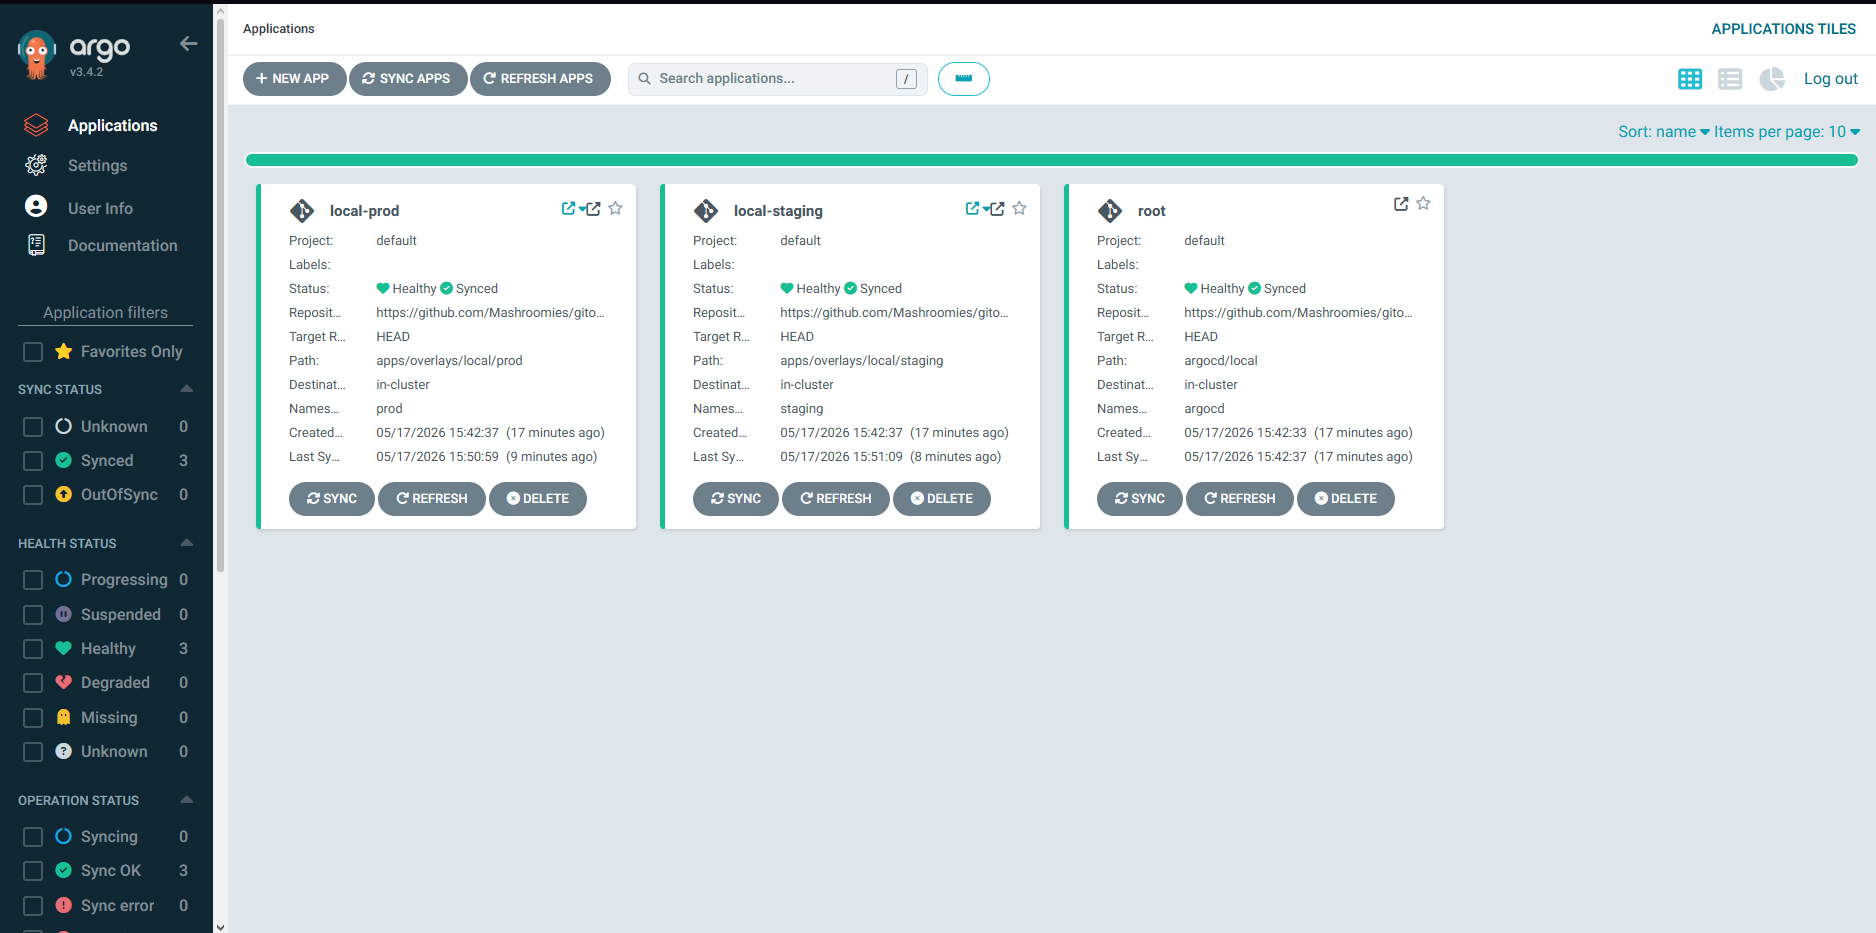
\includegraphics[width=1\linewidth]{src/assets/images/argocd-dashboard.png}
    \caption{ArgoCD dashboard showing all applications healthy and synced}
    \label{fig:argocd-dashboard}
\end{figure}
 
\subsubsection{Running Pods and Services}
Figure \ref{fig:pods-running} shows the ArgoCD resource tree
for the production environment. Incoming traffic enters through
the Ingress, gets routed to each application's Service, and
reaches the corresponding running pod. All three applications,
the API, the Landing Page, and the Studio, are in a healthy
and running state.
 
\begin{figure}[H]
    \centering
    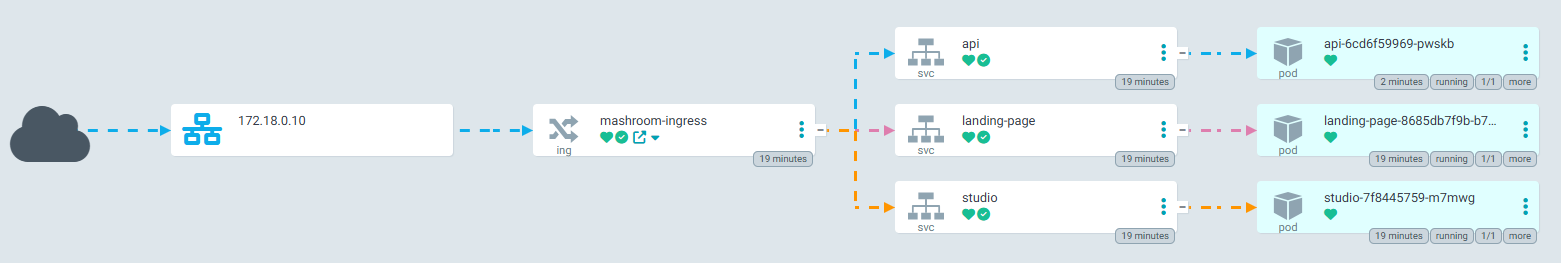
\includegraphics[width=1\linewidth]{src/assets/images/pods-running.png}
    \caption{ArgoCD resource tree showing all pods running and healthy}
    \label{fig:pods-running}
\end{figure}
% ----------------------- Conclusion ----------------------- %
\setcounter{secnumdepth}{0}
\section{Conclusion}
This chapter covered the full implementation of The Mashroom's platform.
Starting from containerizing the applications and configuring the
Kubernetes cluster, to provisioning the AWS infrastructure with Terraform,
and finally setting up the CI/CD pipelines, the result is a fully automated
delivery process where a code change is the only manual step required.
Each stage was validated in place, confirming that the infrastructure,
the pipelines, and the deployment automation all behave as designed.